\section{Background}

\subsection{Settings}

\subsubsection{Bandit Setting}

For simplicity, we first present the main results in the standard bandit setting, and then discuss several general settings.

In the standard bandit setting, we have $n = 1$. At each time step $t$, the agent takes an action $A_t \in [h]$ according to some strategies, and then it observes a reward $r_{A_t} \in \sR$. The agent then uses the reward to improve its action selection strategies. After such $T$ time steps, the performance of the agent's strategy is measured by the (expected) regret,
\begin{equation}
\label{eq:expected_regret}
    \r_i^{\max} \cdot T - \sE \left[ \sum\limits_{t=0}^{T-1}{  r_{i, A_t}  } \right] = \sum\limits_{t=0}^{T-1}{ \sE \left[ \tilde{r}_{i, A_t} \right] },
\end{equation}
where the expectation is taken over the randomness of action selection, if the agent is using stochastic strategies.

Note that we choose to keep the subscript $i$ here to make the later generalization from the bandit case to the many state dependent case smoother, although there is only one state ($n = 1$) thus $i$ can be omitted without ambiguity.

\subsubsection{Episodic Markov decision process (MDP)}

The episodic MDP setting recovers the bandit setting as a special case. The environment randomly select a starting state $\rvs_i^0 \in \sR^d$. At each time step $t$, the agent takes one action $A_t \in [h]$ according to some strategies, and then it observes a reward $r_{A_t} \in \sR$ and next state $S_{t+1} \sim \sP\left( \cdot \middle| S_t, A_t \right)$, where $\sP$ is the transition probability matrix and it is unknown to the agent. After such $H$ steps, the agent observes an ending state $S_H$, and the current trajectory terminates. At the next time step, the agent will observe a new starting state $\rvs_i^0$ randomly generated by the environment. Since we use policy gradient method (no value learning), the agent updates its NN policy weights using the cumulative reward collected after each trajectory terminates.

\subsection{Neural Network (NN) Policy}

The structure of the neural network policy is shown in \cref{fig:nn_policy}. The policy NN takes the feature vector of each state $\rvs_i \in \sR^d$ as the input. Then it calculates the hidden node value vector by $u_{i,r} \triangleq \rvw_r^\top \rvs_i$, $\forall r \in [m]$. The logit vector is calculated by $o_{i,k} \triangleq \rva_k^\top \sigma\left( \rvu_i \right)$, $\forall k \in [h]$, where $\sigma$ is element-wise ReLU activation function. Finally, the policy probability is the softmax transform of the logit vector, i.e., $\rvpi_i \triangleq f\left( \rvo_i \right) = f\left( \rmA^\top \sigma\left( \rmW^\top \rvs_i \right) \right)$. 
\begin{figure}[t]
\vskip 0.2in
\begin{center}
\centerline{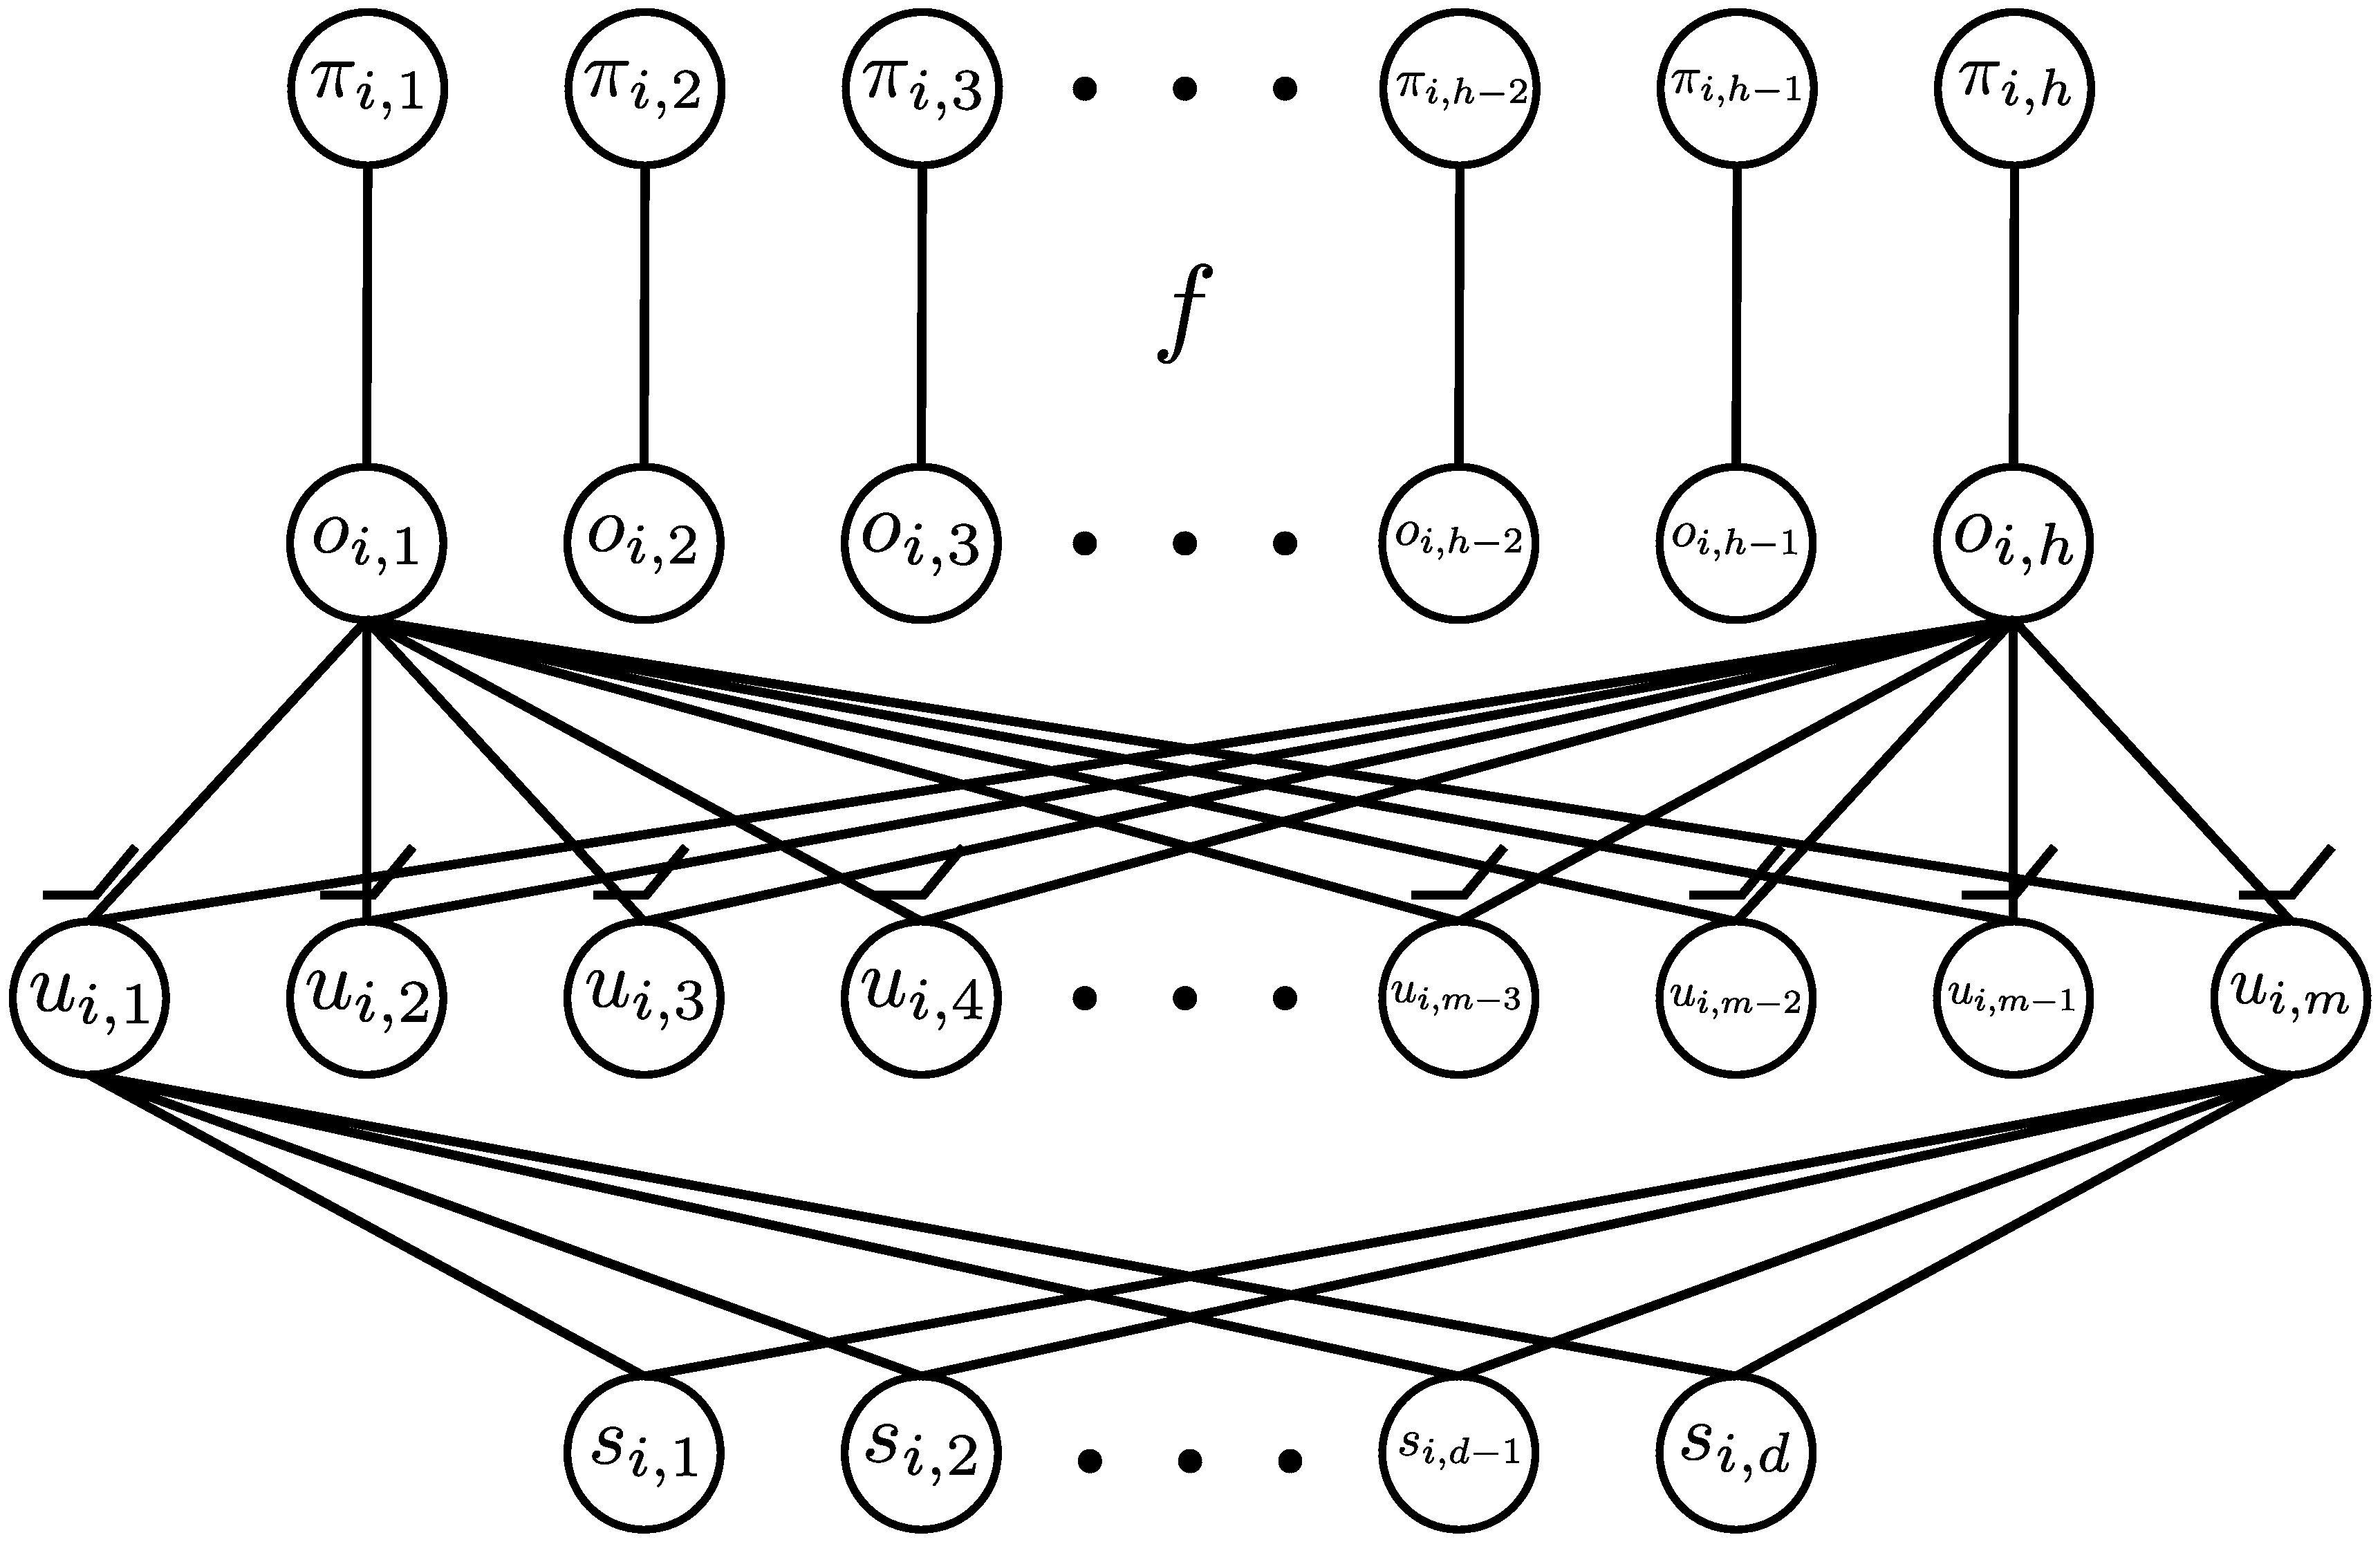
\includegraphics[width=\columnwidth]{nn_policy.pdf}}
\caption{Policy neural network.}
\label{fig:nn_policy}
\end{center}
\vskip -0.2in
\end{figure}

The above neural network defines a family of policies $\rvpi_i \left( \rmW \right)$ parameterized by $\rmW \in \sR^{d \times m}$ given any state $\rvs_i$. Let $\rvpi_i = \rvpi_i \left( \rmW \right)$, the expected loss can be calculated according to \cref{eq:expected_loss}.

\subsection{Vanilla Policy Gradient}
\label{subsec:vanilla_policy_gradient}

During the process of interacting with the environment, the agent can use any strategies to select actions. In particular, if at each time step $t$, the agent's action selection strategy is the NN policy $\rvpi_i(t)$, then the (expected) regret is equivalent to the cumulative expected loss of $\rvpi_i$, i.e., 
\begin{equation}
\label{eq:vanilla_policy_gradient_expected_regret}
\begin{split}
    \sum\limits_{t=0}^{T-1}{ \expectation\limits_{A_t \sim \rvpi_i(t)} \left[ \tilde{r}_{i, A_t} \right] } = \sum\limits_{t=0}^{T-1}{\rvpi_i(t)^\top \rvtilder_i} = \sum\limits_{t=0}^{T-1}{\ell(t)},
\end{split}
\end{equation}
according to \cref{eq:expected_loss} and \cref{eq:expected_regret}. Using \cref{eq:vanilla_policy_gradient_expected_regret}, at each time step $t$, the agent can use the current NN policy $\rvpi_i(t)$ to sample an action, and obtain an estimation of the expected loss $\ell(t)$. Doing policy gradient descent with respect to the NN weights $\rmW(t)$ will arguably decrese the expected loss, thus reduce the expected regret. 

However, the above mentioned method, called as vanilla policy gradient, often suffers the ``lack of exploration" problem in practice, i.e., some actions can never be explored thus cannot be learned. Unfortunately, without any other techniques the vanilla policy gradient method cannot circumvent this issue. Actually, as our proof shown later on, the convergence of policy expected loss relies on non-zero probability of exploring optimal arms, which is consistent with intuition. For this reason, we need mix the vanilla policy gradient method with explicit exploration.

\subsection{Policy Gradient with Uniform Exploration}

A natural way is to add uniform exploration to the policy gradient method, as shown in \cref{alg:policy_gradient_uniform_exploration}. The policy gradient method with uniform exploration works as follows. After the random initialization, at each time step $t$, the learning is performed by updating the NN policy $\rvpi_i(t)$, using the estimated policy gradient calculated from the collected reward. In the first $\sqrt{T}$ steps, actions are sampled subject to an uniform distribution over all actions, which we call it the ``exploring phase". After that, the NN policy $\rvpi_i(t)$ is used to sample actions, called as the ``playing phase".

\begin{algorithm}[t]
   \caption{Policy Gradient with Uniform Exploration}
\label{alg:policy_gradient_uniform_exploration}
\begin{algorithmic}
   \STATE {\bfseries Input:} State feature vectors $\rvs_i$, learning rate $\eta > 0$.
   \STATE Initialize $\rvw_r \sim \gN\left( 0, \sigma^2 \cdot \rmI \right)$, $\forall r \in [m]$, $\rva_k \sim \gN(0, \rmI)$, $\forall k \in [h]$.
   \FOR{$t=0$ {\bfseries to} $T-1$}
   \IF{$t < \sqrt{T}$}
   \STATE (Exploring Phase)
   \STATE Uniformly randomly sample action $A_{t} \in [h]$. 
   \ELSE
   \STATE (Playing Phase)
   \STATE Sample action $A_{t} \sim \rvpi_{i}(t)\left(\cdot \middle| \rvs_i \right)$.
   \ENDIF
   \STATE Take action $A_{t}$.
   \STATE Observe reward $r_{i, A_{t}}$.
   \STATE Calculate estimated loss $\ell(t)$.
   \STATE Update $\rvpi_{i}(t)$ to $\rvpi_{i}(t+1)$ by policy gradient: 
   \STATE $\rvw_r(t+1) = \rvw_r(t) - \eta \cdot \frac{d\ell(t)}{d \rvw_r(t)}$, $\forall r \in [m]$.
   \ENDFOR
\end{algorithmic}
\end{algorithm}

